\documentclass{beamer}
\usetheme{metropolis}
\usefonttheme[onlymath]{serif}
\usepackage{amssymb,amsmath}
\usepackage{minted}
\usepackage{subcaption}

\setbeamertemplate{footline}[frame number]
\setbeamertemplate{navigation symbols}{}


\author{William Maxwell}
\title{An implementation of chordal graph algorithms in FGL}
\date{}

\begin{document}

\begin{frame}
    \titlepage
\end{frame}

\begin{frame}{Overview}
    \tableofcontents
\end{frame}

\section{Chordal graphs}

\begin{frame}{Chordal graphs}
\begin{definition}
A graph is called a chordal graph if every cycle in the graph has a chord.
\end{definition}
\begin{figure}
        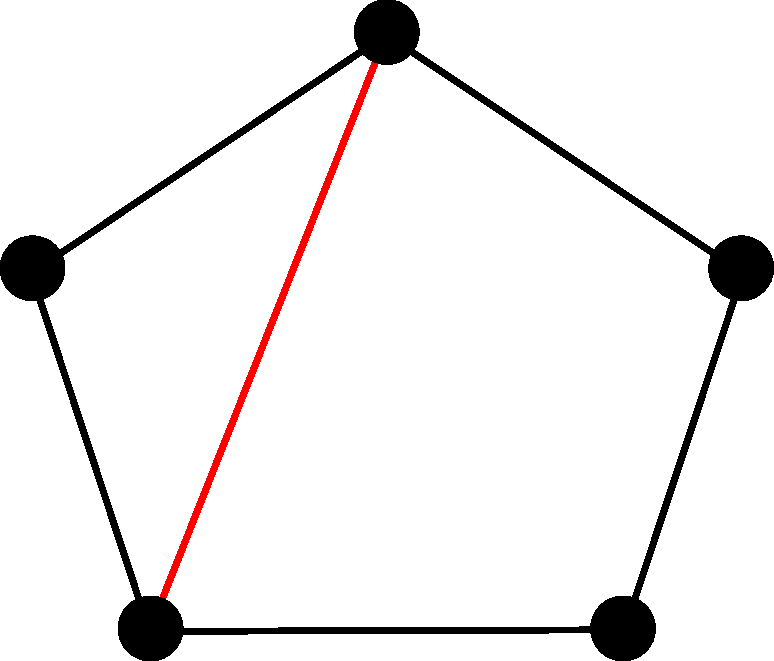
\includegraphics[scale=0.3]{chord.pdf}
        \caption*{The red edge is a chord, but the graph is not chordal}
\end{figure}
\end{frame}

\begin{frame}{Chordal graphs}
\begin{definition}
A graph is called chordal if the vertices can be ordered $v_1,v_2,\dots,v_n$ such that for each $1 \leq i \leq n$, $v_i$ and its neighbors with index greater than $i$ form a clique.
\end{definition}
\begin{figure}
    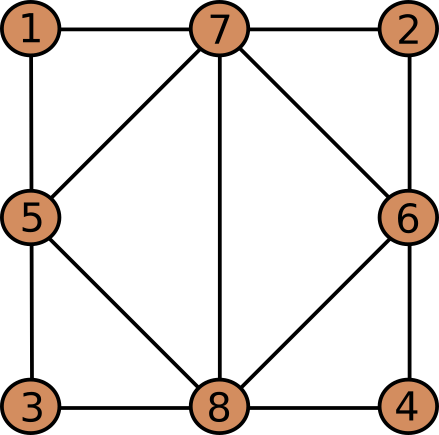
\includegraphics[scale=0.3]{g1107.png}
    \caption*{A chordal graph and its ordering}
\end{figure}
\end{frame}

\begin{frame}{Algorithmic results}
Many \textsf{NP}-Complete problems are polynomial or linear on chordal graphs. A few well known problems include\\

Maximum clique\\
Maximum coloring\\
Maximum independent set\\
Minimum width tree decomposition
\end{frame}

\section{Chordal graphs in FGL}

\begin{frame}[fragile]{Graph data types}
\begin{minted}{haskell}
type Node        = Int
type Adj b       = [(b, Node)]
type Context a b = (Adj b, Node, a, Adj b)
\end{minted}
\begin{minted}{haskell}
data Graph a b   = Empty | Context a b & Graph a b
\end{minted}
In FGL \texttt{Graph} is actually a type class and the constructors are functions required by the implementation of the type class
\end{frame}

\section{Algorithm implementations}

\begin{frame}[fragile]{Maximum clique}
\begin{minted}[fontsize=\footnotesize]{haskell}
-- Compute the size of a maximum clique
maxClique :: Gr a b -> Int                                                           
maxClique g = 1 + ufold (\c k -> max (length $ suc' c) k) 0 g

-- Compute a maximum clique
maxClique :: Gr a b -> [Node]
maxClique = ufold maxClique' []

maxClique' :: Context a b -> [Node] -> [Node]
maxClique' c ns = if length ns' > length ns then ns' else ns
    where ns' = n : suc' c
          n   = node' c

\end{minted}
\end{frame}

\begin{frame}[fragile]{Chordal completion}
\begin{minted}[fontsize=\scriptsize]{haskell}
chordalCompletion :: Gr a () -> Gr a ()                                                      
chordalCompletion g = ufold chordalCompletion' g g

chordalCompletion' :: Context a () -> Gr a () -> Gr a ()
chordalCompletion' c g = addClique g (map fst $ suc' c)


addClique :: Gr a () -> [Node] -> Gr a ()                                                    
addClique g []     = g
addClique g (n:ns) = addClique gc ns
    where gc = insEdges fs g
          es = labEdges g
          fs = [x | x <- zip3 (repeat n) ns (repeat ()), not (x `elem` es)]
\end{minted}
\end{frame}

\begin{frame}[fragile]{Is Chordal?}
\begin{minted}[fontsize=\footnotesize]{haskell}
isChordal :: Gr a b -> Bool
isChordal g = isChordal' g (edges g)

isChordal' :: Gr a b -> [Edge] -> Bool
isChordal' g es
    | isEmpty g = True
    | otherwise = isClique sucs es && isChordal' g' es
        where (c,g') = matchAny g                                                            
              sucs   = suc' c

isClique :: [Node] -> [Edge] -> Bool
isClique [] _ = True
isClique (n:ns) es = checkVertex n ns && isClique ns es
    where checkVertex n [] = True
          checkVertex n (n':ns) = (n,n') `elem` es && checkVertex n ns
\end{minted}
\end{frame}

\section{Tree decompositions}

\begin{frame}{Tree decompositions}
A tree decomposition of a graph $G$ is a tree whose vertices (called bags) are sets of vertices from $G$ satisfying some a few properties\\\\
A tree decomposition tells us how "treelike" our graph is\\\\
Removing a single bag from $G$ disconnects $G$ similar to how removing a single vertex from a tree disconnects the tree\\\\
The size of the largest bag determines the treewidth of a graph
\end{frame}

\begin{frame}{Tree decompositions}
Many \textsf{NP}-Complete problems are efficient on graphs with small treewidth\\\\
Problems are typically solved via dynamic programming on the tree decomposition
\end{frame}

\begin{frame}{An example}
\begin{figure}
    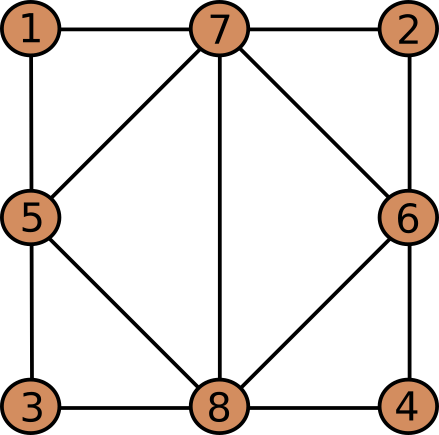
\includegraphics[scale=0.3]{g1107.png}
    \hspace{1cm}
    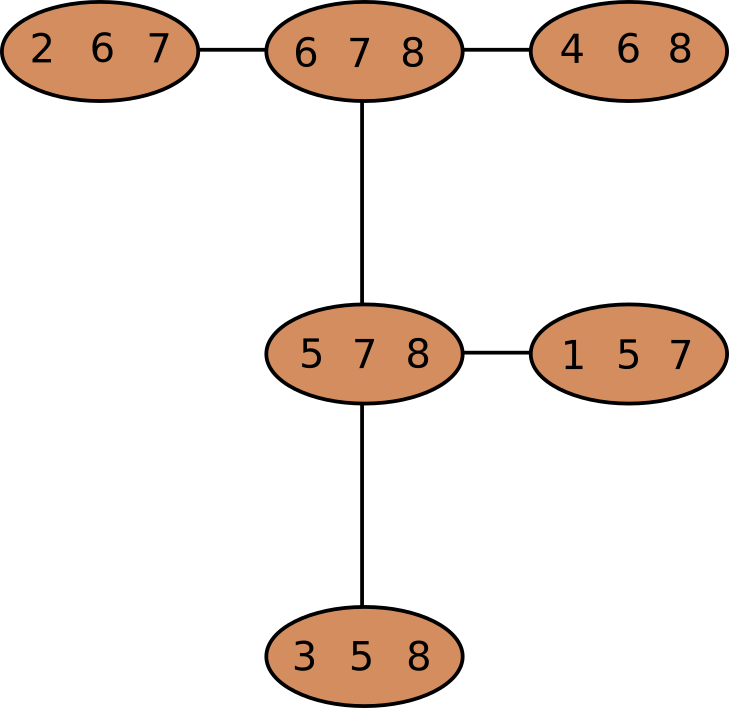
\includegraphics[scale=0.2]{treedecomp.png}
    \caption*{A graph and a tree decomposition}
\end{figure}
\end{frame}

\begin{frame}[fragile]{Tree decomposition types}
\begin{minted}{haskell}
type Bag        = Set Node
type TreeDecomp = Gr Bag ()

\end{minted}
\end{frame}

\begin{frame}{Imperative tree decomposition algorithm}
\begin{figure}
    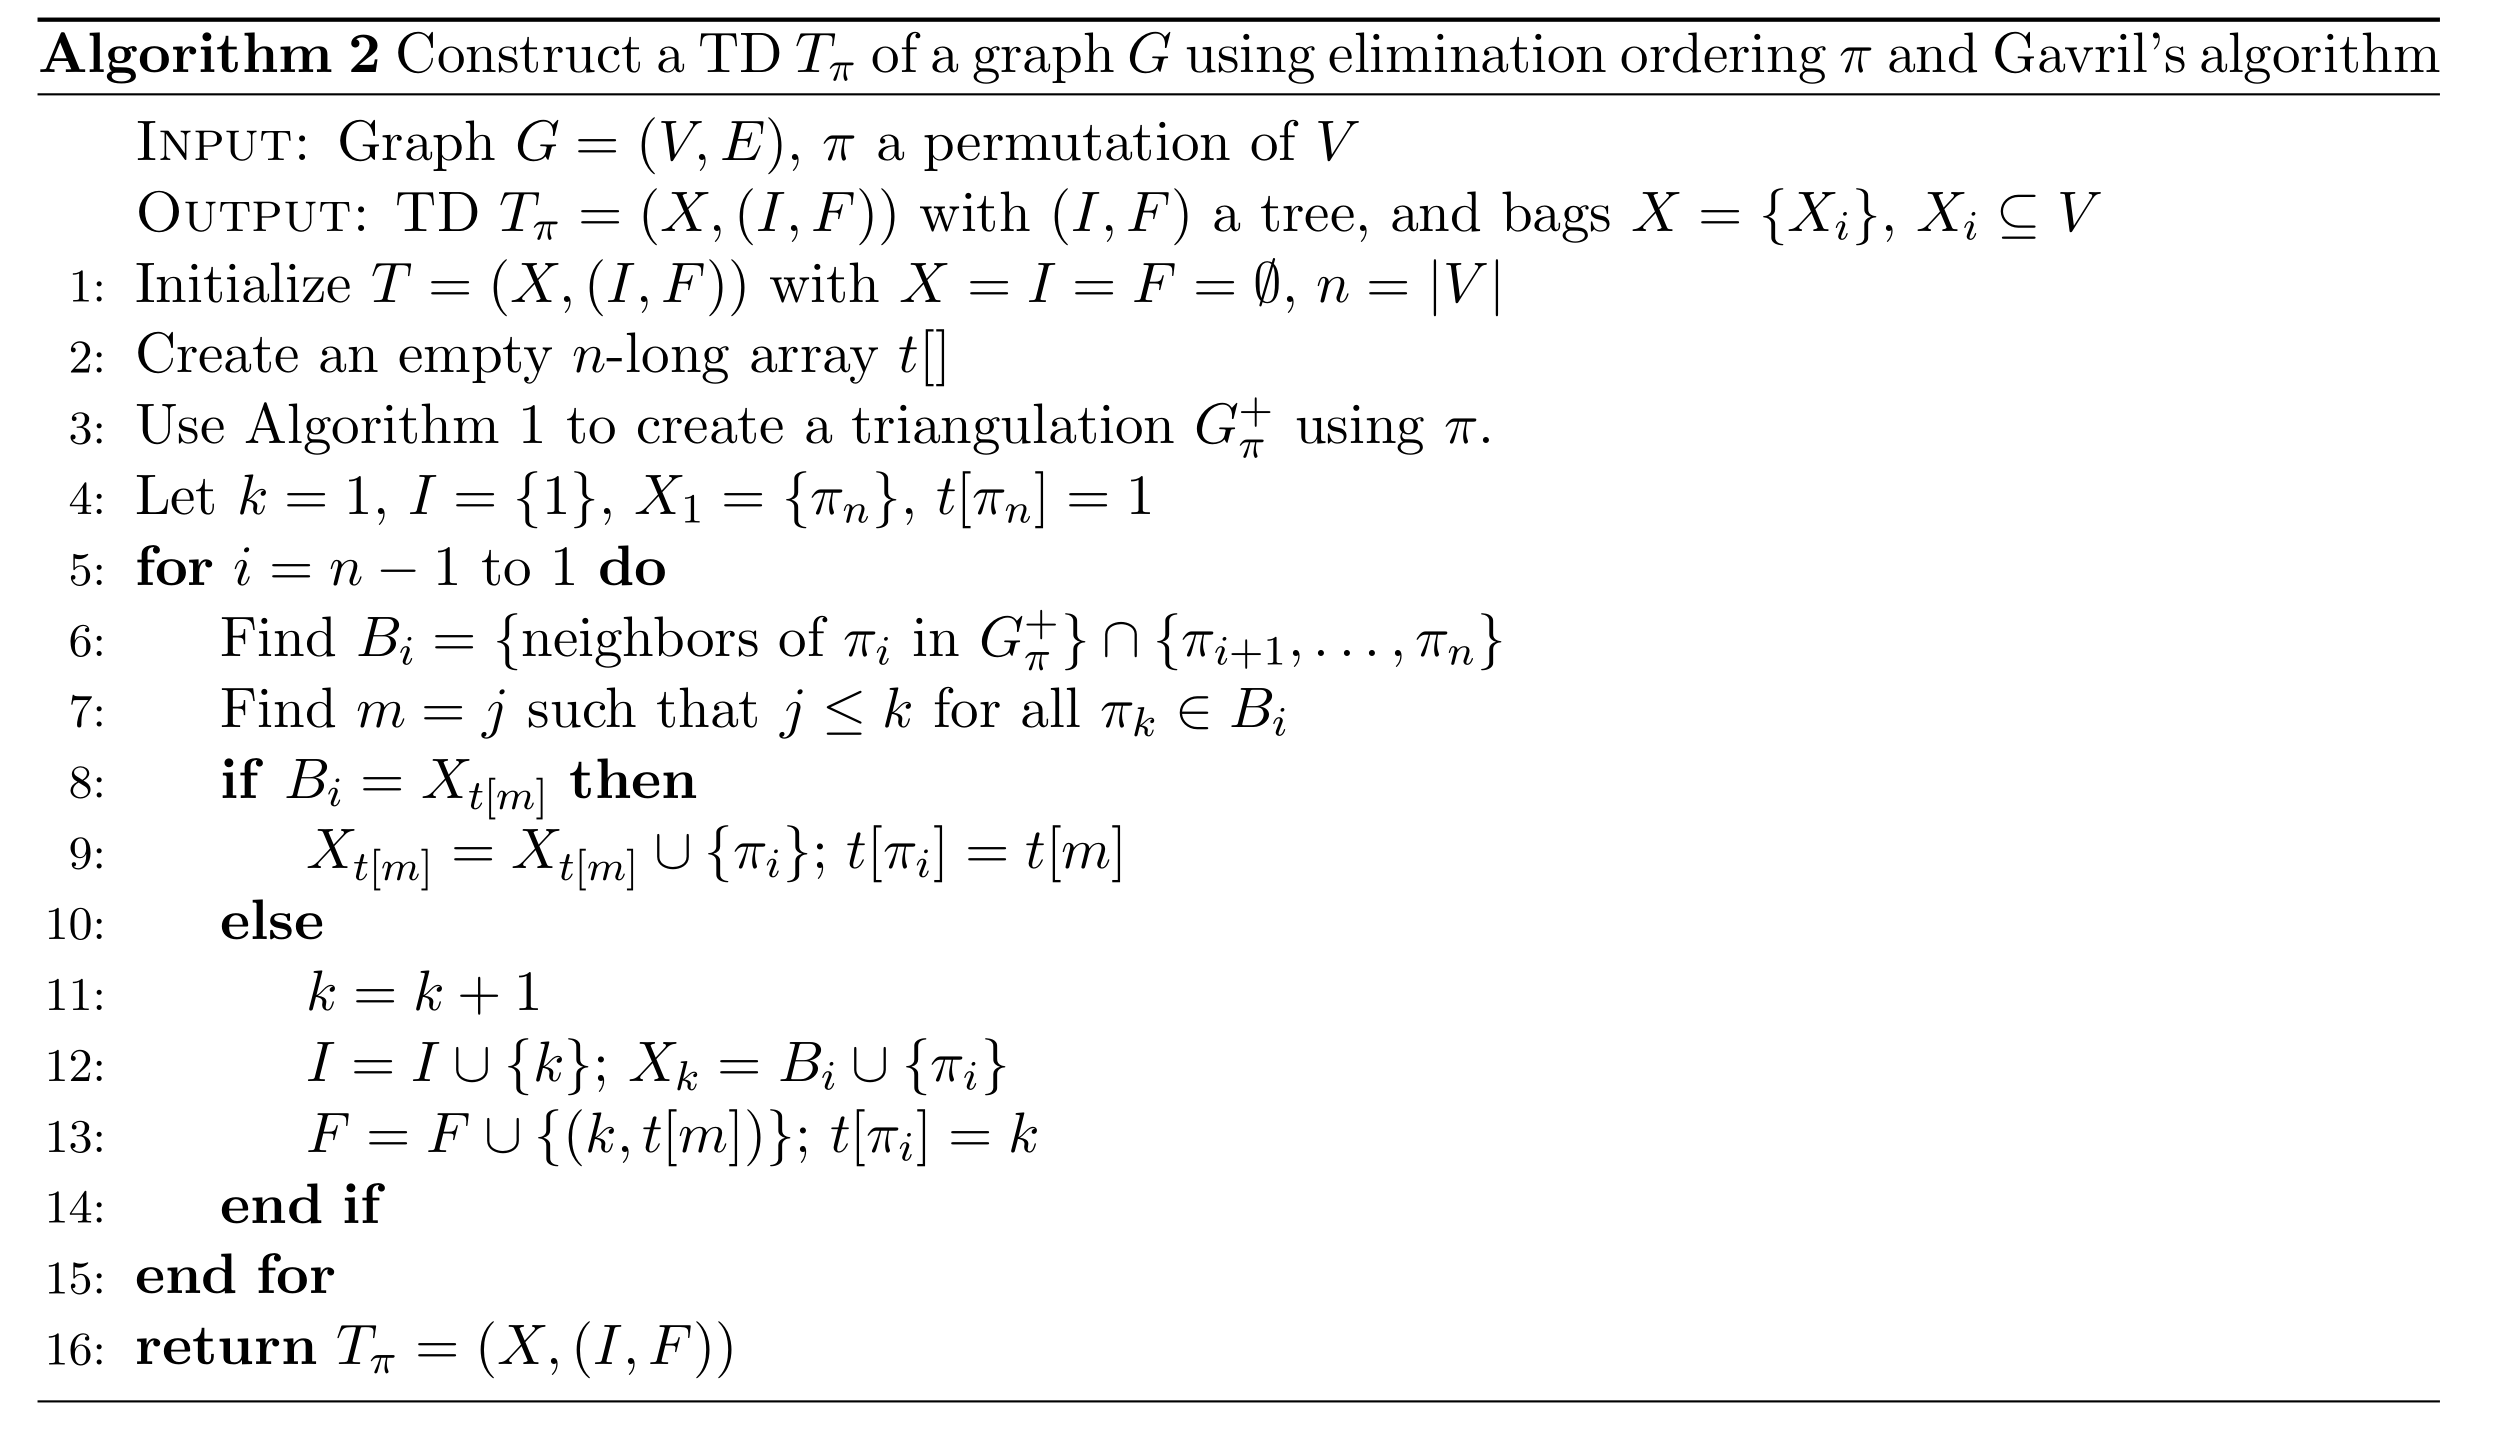
\includegraphics[scale=0.5]{algo.png}
    \caption*{\textit{Aaron B. Adcock and Blair D. Sullivan and Michael W. Mahoney, Tree decompositions and social graphs}}
\end{figure}
\end{frame}

\begin{frame}[fragile]{Tree decomposition types}
\begin{minted}{haskell}
type SucSet     = Node -> Set Node

data TDState = TDState {
    bagMap    :: IntMap Node,
    sucMap    :: SucSet,
    partialTD :: TreeDecomp,
    currBag   :: Node
}

buildTreeDecomp :: Gr a b -> State TDState ()
\end{minted}
\end{frame}

\begin{frame}[fragile]{The SucSet type}
\begin{minted}[fontsize=\scriptsize]{haskell}
addSucs :: SucSet -> Node -> [Node] -> SucSet
addSucs f n ns = \x -> if x `elem` ns then Set.insert n (f x) else f x
        
getSucSet :: Gr a b -> SucSet
getSucSet = ufold (\c f -> addSucs f (node' c) (pre' c)) (const Set.empty)  
\end{minted}
\end{frame}

\begin{frame}[fragile]{Adding a vertex to a bag}
\begin{minted}[fontsize=\footnotesize]{haskell}
-- First node is the bag, second node is the new vertex
addToBag :: TreeDecomp -> Node -> Node -> TreeDecomp
addToBag td b v = insNode (b, lb') (delNode b td)
    where lb  = case lab td b of (Just l) -> l
                                 Nothing  -> error "Bag not found"                           
          lb' = Set.insert v lb
\end{minted}
\end{frame}

\end{document}
